 \documentclass[a4paper,12pt]{article}
 \usepackage[table,xcdraw]{xcolor}
\usepackage[margin=2cm]{geometry}
\usepackage{amsmath}
\usepackage{amsfonts}
\usepackage{graphicx}   
\usepackage{float}
\usepackage[center]{caption}
\usepackage{subcaption}
\usepackage[square,sort,comma,numbers]{natbib}
\usepackage{tikz,pgfplots}
\usepackage{filecontents}
\usepackage{wrapfig}
\usepackage{upgreek}
\usepackage{appendix}
\newcommand{\HRule}{\rule{\linewidth}{0.5mm}}


\tikzstyle{mybox} = [draw=blue, fill=blue!20, very thick,
    rectangle, rounded corners, inner sep=8pt, inner ysep=5pt, text width=10em, minimum height=1em]

\begin{filecontents*}{alphasigma.csv}            
Alpha,Mono,Bis,Tris
0,110,70,100
0.01,90,70,70
0.02,91,66,90
0.03,90,60,50
0.04,88,70,60
0.05,56,30,80
0.06,52,20,40
0.07,33,20,40
0.08,31,20,30
0.09,24,10,30
0.1,17,20,20
0.11,17,8,7
0.12,17,5,3
0.13,7,7,2
0.14,6,0,1
0.15,6,0,1
0.16,4,0,2
0.17,4,0,4
0.18,4,0,2
0.19,6,0,6
0.2,2,0,0
0.21,0,0,0
\end{filecontents*}

\begin{filecontents*}{calculation_of_D.csv}       
ts,rts,mr,mrm,br,brm,tr,trm
0,0,13.24223924,1.32422E-08,11.14983408,1.11498E-08,12.28323247,1.22832E-08
1,2.23607E-08,13.79687646,1.37969E-08,11.14983408,1.11498E-08,12.28323247,1.22832E-08
2,3.16228E-08,14.63582932,1.46358E-08,11.88094693,1.18809E-08,12.28323247,1.22832E-08
3,3.87298E-08,15.01952396,1.50195E-08,12.69841722,1.26984E-08,12.28323247,1.22832E-08
4,4.47214E-08,17.0411766,1.70412E-08,14.96754155,1.49675E-08,15.23701414,1.5237E-08
5,0.00000005,18.94363745,1.89436E-08,16.1439834,1.6144E-08,17.044967,1.7045E-08
6,5.47723E-08,18.22606376,1.82261E-08,15.21834748,1.52183E-08,16.45004863,1.645E-08
7,5.91608E-08,14.68733808,1.46873E-08,8.703757809,8.70376E-09,9.508611886,9.50861E-09
8,6.32456E-08,11.99719134,1.19972E-08,9.202575726,9.20258E-09,11.04810391,1.10481E-08
9,6.7082E-08,11.99719134,1.19972E-08,11.14983408,1.11498E-08,12.28323247,1.22832E-08
10,7.07107E-08,11.99719134,1.19972E-08,11.14983408,1.11498E-08,12.28323247,1.22832E-08
11,7.4162E-08,12.28132322,1.22813E-08,11.88094693,1.18809E-08,12.28323247,1.22832E-08
12,7.74597E-08,14.68733808,1.46873E-08,11.88094693,1.18809E-08,12.28323247,1.22832E-08
13,8.06226E-08,17.16338836,1.71634E-08,14.96754155,1.49675E-08,15.17888665,1.51789E-08
14,8.3666E-08,18.70887757,1.87089E-08,15.98217132,1.59822E-08,16.71047875,1.67105E-08
15,8.66025E-08,19.35339505,1.93534E-08,16.73331408,1.67333E-08,19.05924972,1.90592E-08
16,8.94427E-08,19.81048965,1.98105E-08,17.09174655,1.70917E-08,19.52910648,1.95291E-08
17,9.21954E-08,22.57567718,2.25757E-08,17.31418494,1.73142E-08,19.52910648,1.95291E-08
18,9.48683E-08,23.81809396,2.38181E-08,17.31418494,1.73142E-08,19.52910648,1.95291E-08
19,9.74679E-08,23.81809396,2.38181E-08,17.09174655,1.70917E-08,19.52910648,1.95291E-08
20,0.0000001,23.71639517,2.37164E-08,16.87707913,1.68771E-08,18.33120291,1.83312E-08
21,1.0247E-07,23.13981201,2.31398E-08,16.73331408,1.67333E-08,14.22478119,1.42248E-08
22,1.04881E-07,21.79864675,2.17986E-08,17.09174655,1.70917E-08,13.71444859,1.37144E-08
23,1.07238E-07,21.17394153,2.11739E-08,17.31418494,1.73142E-08,18.33120291,1.83312E-08
24,1.09545E-07,20.04657078,2.00466E-08,17.31418494,1.73142E-08,19.52910648,1.95291E-08
25,1.11803E-07,20.44706336,2.04471E-08,17.31418494,1.73142E-08,19.52910648,1.95291E-08
26,1.14018E-07,25.22064432,2.52206E-08,17.70018361,1.77002E-08,19.52910648,1.95291E-08
27,1.1619E-07,26.04740486,2.60474E-08,20.98299311,2.0983E-08,20.65191759,2.06519E-08
28,1.18322E-07,26.2386928,2.62387E-08,24.22173198,2.42217E-08,25.39206569,2.53921E-08
29,1.20416E-07,26.51659669,2.65166E-08,24.55286949,2.45529E-08,25.83799721,2.5838E-08
30,1.22474E-07,29.34633197,2.93463E-08,24.47043114,2.44704E-08,25.83799721,2.5838E-08
31,1.24499E-07,31.01201864,3.1012E-08,24.22173198,2.42217E-08,25.83799721,2.5838E-08
32,1.26491E-07,30.81500933,3.0815E-08,23.70278887,2.37028E-08,24.5878954,2.45879E-08
33,1.28452E-07,30.48200289,3.0482E-08,23.23154752,2.32315E-08,23.30864861,2.33086E-08
34,1.30384E-07,30.26020489,3.02602E-08,23.10821066,2.31082E-08,22.38875611,2.23888E-08
35,1.32288E-07,29.34633197,2.93463E-08,23.74595966,2.3746E-08,22.38875611,2.23888E-08
36,1.34164E-07,28.84362148,2.88436E-08,24.70077327,2.47008E-08,23.56491884,2.35649E-08
37,1.36015E-07,29.01309532,2.90131E-08,25.02116504,2.50212E-08,26.64103977,2.6641E-08
38,1.3784E-07,32.89888904,3.28989E-08,25.59648804,2.55965E-08,27.07268365,2.70727E-08
39,1.39642E-07,33.58321754,3.35832E-08,26.53383877,2.65338E-08,27.4639054,2.74639E-08
40,1.41421E-07,33.91279699,3.39128E-08,26.75867149,2.67587E-08,28.63217421,2.86322E-08
41,1.43178E-07,34.00382626,3.40038E-08,29.8762347,2.98762E-08,30.91749343,3.09175E-08
42,1.44914E-07,34.91458435,3.49146E-08,30.13723445,3.01372E-08,31.84119816,3.18412E-08
43,1.46629E-07,37.58916067,3.75892E-08,30.06816922,3.00682E-08,30.91749343,3.09175E-08
44,1.48324E-07,37.90004749,3.79E-08,29.80800228,2.9808E-08,29.650715,2.96507E-08
45,0.00000015,37.49866264,3.74987E-08,29.08586255,2.90859E-08,29.31760734,2.93176E-08
46,1.51658E-07,36.69975068,3.66998E-08,28.54635003,2.85464E-08,28.91859436,2.89186E-08
47,1.53297E-07,36.05992374,3.60599E-08,27.96289863,2.79629E-08,28.66407159,2.86641E-08
48,1.54919E-07,35.67208012,3.56721E-08,28.20788188,2.82079E-08,28.66407159,2.86641E-08
49,1.56525E-07,35.67962724,3.56796E-08,30.67891947,3.06789E-08,29.30645492,2.93065E-08
50,1.58114E-07,37.90520545,3.79052E-08,32.3071277,3.23071E-08,32.84439678,3.28444E-08
51,1.59687E-07,39.81071213,3.98107E-08,32.85426304,3.28543E-08,34.44630895,3.44463E-08
52,1.61245E-07,40.65679033,4.06568E-08,32.93497988,3.2935E-08,34.59948844,3.45995E-08
53,1.62788E-07,41.01741459,4.10174E-08,33.23366516,3.32337E-08,34.59948844,3.45995E-08
54,1.64317E-07,41.55607416,4.15561E-08,33.37907578,3.33791E-08,34.44630895,3.44463E-08
55,1.65831E-07,42.9714475,4.29714E-08,33.83791512,3.38379E-08,33.59376877,3.35938E-08
56,1.67332E-07,43.9044713,4.39045E-08,34.1785342,3.41785E-08,33.55643753,3.35564E-08
57,1.68819E-07,43.57535313,4.35754E-08,34.45627519,3.44563E-08,33.55643753,3.35564E-08
58,1.70294E-07,43.13542164,4.31354E-08,34.1785342,3.41785E-08,34.59948844,3.45995E-08
59,1.71756E-07,42.71375657,4.27138E-08,34.15772387,3.41577E-08,34.59948844,3.45995E-08
60,1.73205E-07,42.29809097,4.22981E-08,33.87853155,3.38785E-08,34.59948844,3.45995E-08
61,1.74642E-07,42.26435141,4.22644E-08,34.45627519,3.44563E-08,34.59948844,3.45995E-08
62,1.76068E-07,42.60598197,4.2606E-08,35.49785909,3.54979E-08,34.59948844,3.45995E-08
63,1.77482E-07,44.60104371,4.4601E-08,38.07432468,3.80743E-08,38.05813185,3.80581E-08
64,1.78885E-07,46.63088247,4.66309E-08,39.15909728,3.91591E-08,40.9578039,4.09578E-08
65,1.80278E-07,47.7183099,4.77183E-08,39.15909728,3.91591E-08,40.9578039,4.09578E-08
66,1.81659E-07,48.52753548,4.85275E-08,38.60428603,3.86043E-08,40.81583271,4.08158E-08
67,1.8303E-07,49.21925843,4.92193E-08,37.72372331,3.77237E-08,38.99873844,3.89987E-08
68,1.84391E-07,50.01458387,5.00146E-08,37.05121051,3.70512E-08,37.28938991,3.72894E-08
69,1.85742E-07,50.36554973,5.03655E-08,36.7949059,3.67949E-08,36.50001781,3.65E-08
70,1.87083E-07,49.973534,4.99735E-08,37.02572484,3.70257E-08,36.02957119,3.60296E-08
71,1.88414E-07,49.43358474,4.94336E-08,37.72372331,3.77237E-08,35.91705584,3.59171E-08
72,1.89737E-07,48.8838685,4.88839E-08,39.06410757,3.90641E-08,37.71627235,3.77163E-08
73,1.9105E-07,48.58012145,4.85801E-08,39.55049178,3.95505E-08,39.11276646,3.91128E-08
74,1.92354E-07,48.65013977,4.86501E-08,40.13338511,4.01334E-08,40.9578039,4.09578E-08
75,1.93649E-07,49.70040241,4.97004E-08,41.19410273,4.11941E-08,41.3165318,4.13165E-08
76,1.94936E-07,51.22870387,5.12287E-08,43.5148377,4.35148E-08,41.63600725,4.1636E-08
77,1.96214E-07,52.57058113,5.25706E-08,44.26629756,4.42663E-08,43.25163696,4.32516E-08
78,1.97484E-07,53.44162048,5.34416E-08,44.24082617,4.42408E-08,43.28586028,4.32859E-08
79,1.98746E-07,53.91661525,5.39166E-08,43.6588834,4.36589E-08,42.08020556,4.20802E-08
80,0.0000002,54.25098524,5.4251E-08,42.54400193,4.2544E-08,41.27614929,4.12761E-08
81,2.01246E-07,54.17804906,5.4178E-08,41.28748479,4.12875E-08,40.80506096,4.08051E-08
82,2.02485E-07,53.85004178,5.385E-08,41.05234342,4.10523E-08,40.59200168,4.0592E-08
83,2.03715E-07,53.43514012,5.34351E-08,41.05234342,4.10523E-08,40.87020798,4.08702E-08
84,2.04939E-07,53.19989098,5.31999E-08,41.78438105,4.17844E-08,41.1081987,4.11082E-08
85,2.06155E-07,52.96039275,5.29604E-08,43.97092335,4.39709E-08,41.3165318,4.13165E-08
86,2.07364E-07,53.06148321,5.30615E-08,45.28249551,4.52825E-08,43.28586028,4.32859E-08
87,2.08567E-07,53.43514012,5.34351E-08,46.5108138,4.65108E-08,45.57240064,4.55724E-08
88,2.09762E-07,54.19037368,5.41904E-08,47.38881725,4.73888E-08,46.11585953,4.61159E-08
89,2.1095E-07,55.9008381,5.59008E-08,47.78457492,4.77846E-08,46.02449131,4.60245E-08
90,2.12132E-07,57.76943483,5.77694E-08,47.53448643,4.75345E-08,45.91194507,4.59119E-08
91,2.13307E-07,58.84934494,5.88493E-08,46.58802958,4.6588E-08,44.41632695,4.44163E-08
92,2.14476E-07,59.34215786,5.93422E-08,45.80175324,4.58018E-08,42.6008791,4.26009E-08
93,2.15639E-07,59.25666714,5.92567E-08,45.28249551,4.52825E-08,41.72089405,4.17209E-08
94,2.16795E-07,58.80148468,5.88015E-08,45.08228255,4.50823E-08,41.68051583,4.16805E-08
95,2.17945E-07,57.8509611,5.7851E-08,45.28249551,4.52825E-08,42.08020556,4.20802E-08
96,2.19089E-07,57.1693598,5.71694E-08,45.85661566,4.58566E-08,43.28586028,4.32859E-08
97,2.20227E-07,56.24320492,5.62432E-08,47.02735906,4.70274E-08,44.12136897,4.41214E-08
98,2.21359E-07,56.15162776,5.61516E-08,48.89859098,4.88986E-08,46.02449131,4.60245E-08
99,2.22486E-07,56.97776584,5.69778E-08,50.26840161,5.02684E-08,47.47123971,4.74712E-08
\end{filecontents*}
\pgfplotsset{compat=1.7}

\begin{document}
\begin{titlepage}
\begin{center}


% Upper part of the page  

\textsc{\LARGE Imperial College London}\\[1.5cm]
\centering
\huge Theory and Simulation of Materials\\
M.Sc. Project Report


% Title
\vspace{1.8cm}
\HRule \\[0.4cm]
{ \huge \bfseries Tight-binding approach to the simulation of the electronic and optical properties of porous conjugated molecular materials}\\[0.4cm]

\HRule \\[1.5cm]

% Author and supervisor
\begin{minipage}{0.5\textwidth}
\begin{centering} \Huge
\vspace{1.5cm}
 Beth Rice\\\vspace{2cm}
\large
\emph{Principal supervisor} 
\\
Prof Jenny Nelson\\\vspace{0.5cm}
\emph{Co-supervisors}
\\
Dr Jarvist Frost and Dr Kim Jelfs\\\vspace{1.25cm}
\end{centering}
\end{minipage}
\small
\vfill
A thesis submitted in partial fulfilment of the requirements for the degree of Master of Science of Imperial College London.
\\

% Bottom of the page
\end{center}
\end{titlepage}

\begin{abstract}
\noindent The electronic properties of the different adducts of organic semiconductor PCBM ([6,6]-phenyl-C$_{61}$-butyric acid methyl ester) are investigated with tight-binding methods. The localisation of the charge through energetic disorder and polaronic self-trapping is studied and it is shown that these effects cause the lowest states to be localised to one PCBM molecule. This informs the charge transport models that are explored: wavefunction propagation and charge hopping between polaron states. The former gives the charge mobilities of each adduct in the order expected based on experimental work, although they are much greater which is attributed to the lack of energetic disorder and polaronic effects in the simulation. Weak coupling between polaron states is shown to hold for this system so the latter model is valid. Hopping rates calculated from this reflect the experimental order of mobilities, and pave the way for future work to fully determine the mobilities. 

\end{abstract}


%Contents
\newpage
\tableofcontents
\newpage

%Introduction
\section{Introduction}

\noindent Organic semiconductors (OSCs) based on porous conjugated molecular materials have attracted interest due to their processing advantages and unique properties. Compared to inorganic semiconductors, they are low cost, flexible and easily proccessible from solution \cite{Kwiatkowski2008}. OSCs have applications in optoelectronic devices such as OLEDs, thin film transistors and organic photovoltaics (OPVs). However, efficiencies of devices based on OSCs have not been reached that compete with their inorganic counterparts, and research into them is driven by the prospect of low cost, large-scale production \cite{Hoppe2011}. \\ 

\noindent The performance of optoelectronic devices is determined by the electronic transport properties of OSCs, which are modified for different chemical structures \cite{He2010} \cite{Lenes2009} \cite{Liu2013}. Therefore, good models of charge transport that take into account the physical and chemical properties of OSCs are needed. Predictive models of this kind would pave the way for the design of new materials with favourable properties and improved efficiencies in devices. \\ 

 \noindent The chemical and physical properties of OSCs determine their electronic properties. For OSCs based on fullerene derivatives, strong covalent bonds within molecules and weaker Van der Waals forces between them, as well as the molecular packing and disorder, result in charge states that are relatively localised. The focus of this study will be fullerene derivative PCBM, which has applications in OPVs, as described in Section 1.1 below. The different adducts (mono-, bis- and tris-PCBM) present an opportunity to investigate the effect of molecular packing and structural disorder, and the different isomers of bis- and tris-PCBM exhibit energetic disorder which can also be investigated.\\ 

\noindent The mobility of charge carriers is a crucial measure of the efficiency of an OPV, and it can be found theoretically through modelling the charge transport in a system.  If the charge is localised to one molecule and there is weak electronic coupling between molecules, a hopping model for charge transport can be used \cite{Nelson2009} \cite{Frost2006} \cite{Fishchuk2003}. However, PCBM is a system where weak coupling has been thought not to be valid \cite{Cheung2010} \cite{Oberhofer2012} \cite{Gajdos2013}. Therefore, the more complicated electronic landscapes in this system will be investigated to find a model for charge transport that is applicable. \\

\noindent Modelling charge transport in OSCs is an intrinsically multiscale problem, since the processes involved span a range of length and time scales. A tight-binding approach will be applied to course-grained structures to study the density of states and the delocalisation of charge states under different conditions: structural disorder from the molecular packing of the different adducts, energetic disorder from different isomers and the self-trapping of the charge through interaction with its surroundings. The results of this will be used to find an appropriate model for charge transport, which will be used to find charge mobilities.


\subsection{System of interest}

\noindent PCBM ([6,6]-phenyl-C$_{61}$-butyric acid methyl ester) is a partially disordered fullerene-based material that is used as an electron acceptor in OPVs. There are three adducts of PCBM: mono-, bis- and tris-, which have one, two and three side-chains respectively. Figure \ref{fig:PCBM} shows the chemical structure of mono-PCBM. It is used in OPVs because it is relatively inexpensive, easily processable from solution and can form segregated phases with polymer donors, such as P3HT \cite{Cheung2010}.\\ 

\noindent An OPV is usually made up of an electron donor polymer and an electron acceptor small molecule, which is often based on a fullerene molecule, like PCBM. Both of these have a large conjugated system, where the alternating double and single bonds between carbon atoms form delocalised $\pi$ and $\pi^*$ orbitals which are the HOMO (highest occupied molecular orbital) and LUMO (lowest unoccupied molecular orbital) respectively. The energy difference between these is the band gap of the material \cite{Bredas2004}, and having corresponding donor and acceptor LUMOs improves the performance of the device. \\ 

\noindent The LUMO energy in PCBM is raised by the additional side-chains in bis- and tris-PCBM, which increases the open-circuit voltage, but inhibits close packing of the structures and introduces disorder due to the different isomers, lowering mobility \cite{Lenes2009} \cite{Frost2010}.    

\begin{figure}[H]
\begin{center}
\includegraphics[width=0.7\textwidth]{mono-PCBM.pdf}
\end{center}
\caption{Chemical structure of mono-PCBM \cite{flopic}}
\label{fig:PCBM}
\end{figure}

\noindent The starting point for investigations into these structures will be molecular dynamics simulations that were performed by Dr Jarvist Frost on course-grained PCBM molecules \cite{Steiner}. The system consists of N=1000 course-grained mono-, bis- and tris- PCBM molecules, where the course-graining identified the C$_{60}$ as one grain and each of the side chains as additional grains; this is shown schematically for bis-PCBM in Figure \ref{fig:CG}.

\begin{wrapfigure}{L}{0.5\textwidth}
\begin{center}
\includegraphics[width=0.4\textwidth]{CG-PCBM.pdf}
\end{center}
\caption{The grains for course-graining in MD simulations, shown schematically for bis-PCBM \cite{bispcbm}}
\label{fig:CG}
\end{wrapfigure}


\subsection{Theoretical background}

\noindent One measure characterising the electronic properties of a system is its density of states (DOS). The shape of the DOS for simple 1D, 2D and 3D systems is well-known \cite{Thorpe} and the effect of disorder on the DOS has been well studied for simple systems, where it is found to result in a spreading of the DOS. It has has also been explored in more complicated systems with the low energy `tail' of the DOS being of interest because charges can be trapped in these low energy states, inhibiting charge transport and reducing mobility \cite{Savoie2014a} \cite{Fehske2006} \cite{Welborn2012}. \\

\noindent Tight-binding (TB) approaches have previously been used to study the electronic properties of OSCs \cite{Prins2006} \cite{Mizes1995}. The TB Hamiltonian is formed with site energies on the diagonal and couplings between sites on the off-diagonal and it can be solved to yield the energies and wavefunctions of states. This approach has also been applied to polarons \cite{Molecular-crystal1959} \cite{Klamt1987}. \\ 

\noindent  A polaron is a quasiparticle formed of a conduction electron (or hole) together with its self-induced polarisation in a semiconductor \cite{Devreese1996}. They are of interest in the field of OPVs because electrons involved in charge transport can form polarons \cite{Savoie2014} and they can be delocalised over a number of molecules due to the coupling between the molecules. However, there are various mechanisms that will localise them \cite{PolaronBook}.\\

\noindent Some of the first theoretical studies of charge and polaron localisation were performed by Anderson in the 1950s \cite{Anderson1956}. He showed that introducing static disorder to the site energies leads to localisation. Later, it was shown by Lifshitz \cite{Lifshitz} that the same is true if disorder is introduced to the electronic couplings between sites. Both of these mechanisms have been explored further, including in OPVs \cite{CTDisordered} \cite{Fishchuk2003} \cite{Frost2010} \cite{Troisi2006} \cite{Grozema2002}. In this paper, site energy disorder will be explored directly and electronic coupling disorder will be explored through disorder in the distances between molecules. In addition, mono-, bis- and tris- PCBM will be compared to see effect of strutural disorder due to side chains.\\ 

\noindent Another mechanism for localisation is the `self-trapping' induced by polaron formation, which is described by Holstein for his molecular crystal model \cite{Molecular-crystal1959}. This is when the presence of an electron at one point causes the electron clouds of the surrounding atoms to deform to new equilibrium positions which will be such that a potential well for the electron is formed. This is thought to cause localisation \cite{Fehske2006}. Once the nature of the charges has been found, charge transport models can be applied. \\

\subsection{Previous approaches to charge transport}

\noindent In inorganic semiconductors, charge transport is usually modelled as band transport, but this is not applicable to OPVs since they generally lack the periodicity necessary for this model. In OPVs, it has been simulated using a hopping model, where charge is modelled as localised on one site and hopping to other weakly coupled sites \cite{Nelson2009} \cite{Frost2006} \cite{Fishchuk2003}. Where the weak coupling approximation is not valid, charge transport has been modelled by directly propagating the wavefunction in time \cite{Prins2006} \cite{Grozema2002}.\\ 

\noindent In the weak coupling limit, the rate of hopping can be calculated with the semi-classical Marcus equation. The hopping rate given by Marcus theory is \cite{Marcus1956} 

\begin{equation}
\Gamma_{ij} = \frac{|J_{ij}|^2}{\hbar} \sqrt{\frac{\pi}{\lambda k_B T}} exp \left ( - \frac{(\Delta E_{ij} + \lambda ) ^2}{4\lambda k_B T} \right)
\end{equation}

\noindent where $\Gamma_{ij}$ is the rate of hopping between sites $i$ and $j$, $J_{ij}$ is the electronic coupling between these sites, $\lambda$ is the reorganisation energy and $\Delta E$ is the energy difference between the initial and final states. The condition for weak coupling is that $|J|\ll \lambda$. \\

\noindent Figure \ref{fig:Marcus} shows $\lambda$ and $\Delta E$ with potential energy curves of the two molecules involved in the hop, plotted against the reaction coordinate $Q_r$. The reorganisation energy is the energy relaxation cost in the molecules involved in the hop and their surroundings. It is due to nuclear and electronic reorganisation and is likely to be dominated by electronic polarisation of the environment \cite{Nelson2009}. $\Delta E$ is the energy difference between the inital and final states and $J_{ij}$ is the coupling between states $i$ and $j$.

\begin{figure}[H]
\centering
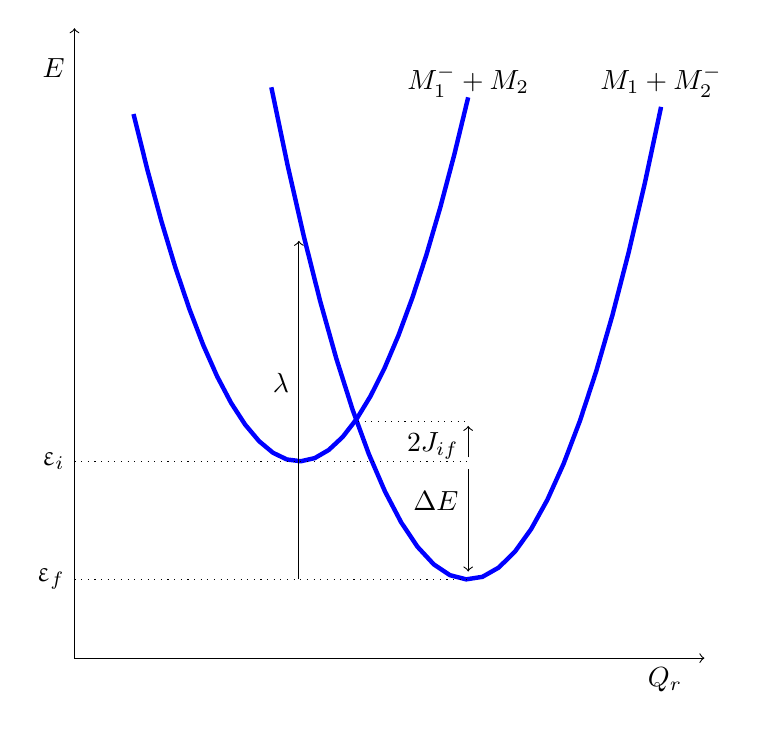
\begin{tikzpicture}
\draw[->] (0,0) -- (8,0);
\draw[->] (0,0) -- (0,8);
\draw (7.5,0) node[below] {$Q_r$};
\draw (0,7.5) node[left] {$E$};
\draw[ultra thick,color=blue,domain=0.75:5] plot (\x, {(\x-2.85)^2+2.5}) ;
\draw[ultra thick,color=blue,domain=2.5:7.45] plot (\x, {(\x-5)^2+1}) ;
\draw[-, dotted] (0,2.5) -- (5,2.5);
\draw[-, dotted] (0,1) -- (5,1);
\draw[-, dotted] (3.6,3) -- (5,3);
\draw[->] (2.85,1) -- (2.85,5.3);
\draw[->] (5,2.4) -- (5,1.1);
\draw[->] (5,2.55) -- (5,2.95);
\draw (2.85,3.5) node[left] {$\lambda$};
\draw (5,2) node[left] {$\Delta E$};
\draw (5,2.7) node[left] {$2 J_{if}$};
\draw (5,7) node[above] {$M_1^- + M_2$};
\draw (7.45,7) node[above] {$M_1+M_2^-$};
\draw (0,1) node[left] {$\upvarepsilon_f$};
\draw (0,2.5) node[left] {$\upvarepsilon_i$};
\end{tikzpicture}
\caption{Potential energy curves for M$_1^- + M_2$ and M$_1+M_2^-$ where $Q_r$ is the reaction coordinate and E is the energy. $\lambda$, $\Delta E$ and $2J$ are shown on the curves.}
\label{fig:Marcus}
\end{figure}

\noindent The Marcus equation yields a set of rates for hopping between all possible sites. The steady state master equation of rates can be used to find the mobility, or the charge can be propagated through the system using kinetic Monte Carlo. This method was applied to C$_{60}$ and P3HT by Nelson \textit{et al} (2009) \cite{Nelson2009}. \\

\noindent In systems that are not weakly coupled, charge has also been propagated through a system by directly evolving the wavefunction of the charge in time with

\begin{equation}
\psi(t) = \sum_k a_k e^{-iE_kt/\hbar} \phi_k,
\label{eq:time}
\end{equation}

\noindent where $\psi(t)$ is the wavefunction at time $t$, $E_k$ and $\phi_k$ are the eigenvalues and eigenvectors of the unperturbed Hamiltonian $H$ and the coefficients $a_k$ are defined as

\begin{equation}
a_k=\langle \phi_k , \psi \rangle,
\end{equation}

\noindent where $\psi$ is the wavefunction to be evolved.\\ 

\noindent This method has been used for propagating the charge in molecular wires \cite{Prins2006}, with the mobilities found compared to experiment. They were 3 orders of magnitude larger than experimental values, which was attributed to the presence of defects and not having an infinite chain. \\

\noindent PCBM has been the subject of many recent papers, due to its interesting properties and potential applications \cite{Savoie2014a} \cite{Albrecht2014} \cite{Frost2010}. Previous models of charge transport in this system have mainly been based on hopping without including polaronic effects, although some studies concluded the system was not weakly coupled so this was not valid \cite{Cheung2010} \cite{Oberhofer2012} \cite{Gajdos2013}. In this study, the degree of localisation through different mechanisms is explored and appropriate models for charge transport are investigated.

\subsection{Approach}

The aim of this study is to develop a course-grained treatment of charge transport in PCBM that takes into account molecular packing, disorder, polaronic effects and the presence of localised and delocalised states within it. To develop a model for this, the density of states and the size of the charge state or polaron will first be investigated using tight-binding methods, with localisation mechanisms being explored as part of this. The results of these will motivate the methods for simulating charge transport, whether it be using an evolution of the wavefunction or a hopping mechanism as described by Marcus theory \cite{Marcus1956}.\\

\noindent Tight-binding methods will be applied to the course-grained structures to get information about the electrical properties of PCBM. As part of this, disorder in couplings and energies will be explored along with the effect of self-trapping of the polaron, which are all known to lead to localisation of the charge \cite{Bronold2002} \cite{Lifshitz}. The resultant wavefunction will be propagated in time to see the movement of the charge and a diffusion constant will be calculated from this. Marcus theory for hopping will also be applied to localised polaron states to model the transport of charge and obtain a set of rates for hopping.

\section{Methods}

\subsection{Tight-binding simulations}

\noindent The NxN tight-binding Hamiltonian has the site energies along the diagonal. Initially, these were all set to the LUMO energy of PCBM for the relevant adduct: -3.7eV for mono-PCBM, -3.56eV for bis-PCBM and -3.49eV for tris-PCBM \cite{Frost2010a}. The off-diagonal elements $H_{ij}, i\neq j$ are populated by the couplings between molecules $i$ and $j$. The positions from the MD simulation were read in and the distance between each molecule and every other molecule was calculated, subject to a maximum cut-off distance and periodic boundary conditions. The coupling $t_{ij}$ was then calculated by \cite{Steiner}:

\begin{equation}
 t_{ij}=t_0 \exp (- \beta d), 
 \label{eq:J}
\end{equation} 
 
\noindent where $t_0$ is the coupling constant, $\beta$ is a characteristic distance and $d$ is the distance between molecules. The eigenvalues of the Hamiltonian are the expectation energies of each state and the corresponding eigenvector squared gives the relative occupation of each site.\\

\noindent A histogram of the eigenvalues represents the density of states (DOS) of the system. The DOS is a key transport parameter for amorphous devices since charges can be trapped in the low energy states, inhibiting transport and reducing mobility \cite{Frosta}. Experimental studies have indicated the presence of a tail in the low energy region of the DOS in OSCs, which has been approximated by an exponential \cite{Cody1981}:

\begin{equation}
N(E)=N_0\exp \left (\frac{E-E_c}{E_{ch}} \right),
\end{equation}

 \noindent where $E_c$ is the mobility edge (the energy at which electrons start moving), $N_0$ is the number of states per volume and $E_{ch}$ is the characteristic energy of the tail. A larger $E_{ch}$ means a larger tail and therefore more trapping of charges. This important parameter was calculated for each adduct of PCBM by fitting an exponential to the low energy tail.
 
 
\subsection{Localisation}

\noindent The PCBM system exhibits intrinsic disorder due to variations in distances between molecules, and therefore there is disorder in couplings. Since the second (and third) side-chains in bis- (and tris-) PCBM can be bonded at different points of the fullerene cage, there are different isomers of each of these available. These different isomers result in energetic disorder in the site energies, which has been included by distributing the site energies normally with the level determined by the standard deviation $\sigma$. The energy distributions due to different isomers have previously been calculated using DFT \cite{Frost2010a}, and when approximated by a Gaussian found to have a standard deviation of $\sigma=$ 56meV and $\sigma=$ 121meV for bis- and tris-PCBM respectively. \\

\noindent  The other mechanism for charge localisation explored is the `self-trapping' effect. This is when stabilisation caused by polaron formation causes a deepening of the energetic states. This was modelled with a self-consistent polaron generator in the code: for a chosen state (the lowest state for initial simulations), electron density for a given site causes deepening of the the site energy, in proportion to the electron density, repeated until convergence of the energy. On each iteration, each site energy is shifted by $\upvarepsilon_i \rightarrow \upvarepsilon_i-\alpha |\psi_i|^2$ and this is shown schematically in Figure \ref{fig:scp}. The proportionality constant $\alpha$ is the binding energy of the polaron localised to a volume of radius $r_p$, given by \cite{tssp} 

\begin{equation}
\alpha=\frac{1}{2}\frac{1}{4\pi}\frac{e^2}{r_p} \left ( \frac{1}{\upvarepsilon_\infty}-\frac{1}{\upvarepsilon_s} \right ), 
\label{eq:alpha}
\end{equation}\\

\noindent where $\upvarepsilon_s$ and $\upvarepsilon_\infty$ are the static and optical dielectric constants respectively and $e$ is the charge on an electron. \\

\begin{figure}[H]
\centering
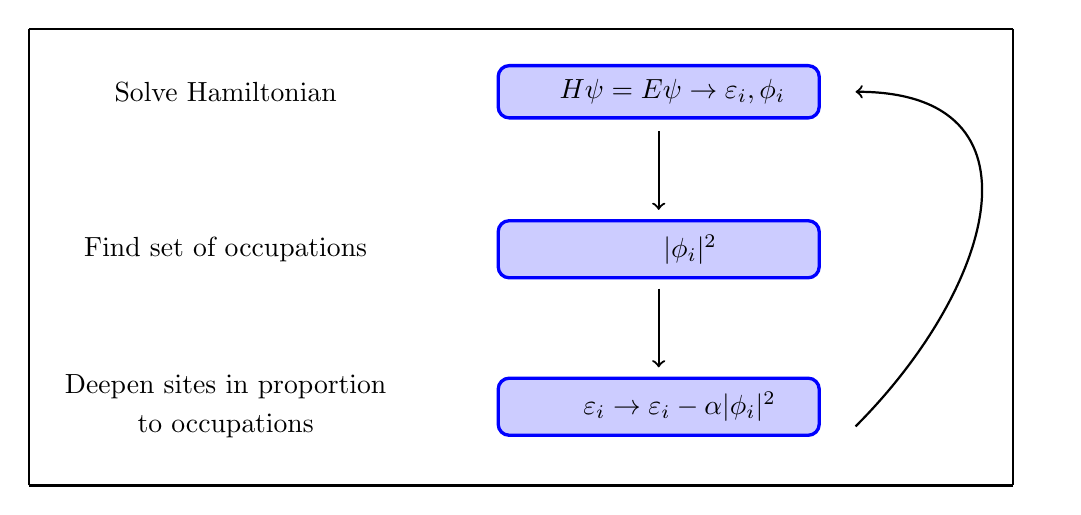
\begin{tikzpicture}
\draw [-, thick] (-2.5,5.8)--(10,5.8);
\draw [-, thick] (10,5.8)--(10,0);
\draw [-, thick] (10,0)--(-2.5,0);
\draw [-, thick] (-2.5,0)--(-2.5,5.8);
\node at (0,5) {Solve Hamiltonian};
\node [mybox] (box) at (5.5,5) {\hspace{0.5cm}$H\psi=E\psi \rightarrow \varepsilon_i,  \phi_i $};
\draw [->,thick] (5.5,4.5) -- (5.5,3.5);
\node at (0,3) {Find set of occupations};
\node  [mybox] (box) at (5.5,3) {\hspace{1.7cm} $|\phi_i|^2$};
\draw [->,thick] (5.5,2.5) -- (5.5,1.5);
\node at (0,1.25) {Deepen sites in proportion};
\node at (0,0.75){to occupations};
\node [mybox] (box) at (5.5,1){\hspace{0.8cm}$\varepsilon_i\rightarrow \varepsilon_i-\alpha|\phi_i|^2$};
\draw [thick](8,0.75) edge[->,out = 45, in = 0, looseness=1.5] (8,5);
\end{tikzpicture}
\caption{An explanation of the self-consistent polaron generator used in the code}
\label{fig:scp}
\end{figure}

\noindent The metric used to measure the extent of localisation was an effective size of the polaron, which was calculated by choosing the most highly occupied molecule as the centre and finding the radius from this within which a given fraction of the charge, chosen to be 99\%, was contained. The number of molecules the polaron is localised over was also estimated by summing all molecules that contained over 1\% of the total charge and this was calculated for the first 10 energy levels.\\

\noindent These two localisation mechanisms were investigated separately as well as together over reasonable ranges based on calculations and previous work. The magnitudes of each needed to localise the lowest state electron density to one molecule was found for all PCBM systems. The self-consistent polaron generator was applied to the system using every state occupation ($|\phi_i|^2$) to get a set of N localised polaron states. The results of these investigations informed the choice of charge transport method.\\

\subsection{Charge transport}

\noindent The charge transport model used depends on the strength of the electronic coupling between molecules ($J$), the size of the charge state or polaron and the local electron-phonon coupling, also called the reorganisation energy ($\lambda$). The methods that were used to simulate charge transport were wavefunction propagation and hopping. 

\subsubsection{Wavefunction propagation} 

\noindent The time evolution of a wavefunction is given in Section 1.3. In this study, $\psi$ was chosen as the wavefunction of the lowest state when it is localised on one molecule, as a result of perturbing the Hamiltonian with polaronic self-trapping effects detailed above. A time-step of 0.1 femtosecond was chosen and the wavefunction was evolved with equation \ref{eq:time}. The electron density diffuses outwards from the molecule: the normalised solution of the diffusion equation for a point source in 3D space is \cite{Bokstein}

\begin{equation}
f(\textbf{r},t) = (4\pi Dt)^{-\frac{3}{2}} \exp \left ( \frac{-\textbf{r}^2}{4 D t} \right ),
\label{eq:diff}
\end{equation}\\

\noindent where $D$ is the diffusion coefficient. The solution of equation (\ref{eq:diff}) is an expanding spherical wave of radius proportional to $\sqrt{4Dt}$. To find the diffusion coefficient numerically, the molecule containing 99\% of the charge was set as the centre of the sphere. Then the charge in spheres of incremental radii $r$ was summed for each time-step, $dt$, for many simulations with different starting configurations of the system, and a histogram was plotted for each $dt$. The diffusion coefficient was extacted from a plot of $r_c$ versus $\sqrt{t}$, where $r_c$ is the radius from the centre containing a fraction of the charge, chosen to be 99\%, and $D$ was found from the gradient of this plot.\\ 


\subsubsection{Hopping model}

\noindent After localising the polaron with the methods described in Section 2.2, the charge transport was also modelled by a hopping mechanism, where valid, between polaron states on different molecules. The polaron states were found by applying the self-consistent polaron generator N times with all N state occupancies to localise it onto N sites. However, some sites were preferred and had multiple occupancy, while many sites were not localised on, so the N sites were not distinct and some sites were therby excluded from the calculation of the rates. For this calculation, replicas of the same polaron state were excluded leaving a set of less than N distinct, non-orthogonal states which take part in transport. The parameters needed for this are the coupling between polaron states $J$, the reorganisation energy $\lambda$ and the energy difference $\Delta E$.\\

\noindent The rates for charge hopping between these polaron states were calculated using Marcus theory as described in Section 1.3 (equation 1). The parameters for this equation are found in the following way: 

\begin{itemize}
\item Reorganisation energy, $\lambda$

\noindent $\lambda$ is given by the sum of the inner ($\lambda_i$) and outer ($\lambda_o$) reorganisation energies, where $\lambda_i$ is the  energy associated with the relaxation of the molecules and $\lambda_o$ is the energy associated with the relaxation of the surrounding medium, folllowing the hop. In this study, it is approximated as $\lambda=2\alpha$, which is true for hopping between identical sites \cite{Duhm2012}. 
 
 \item Electrostatic coupling, $J_{ij}$
 
 \noindent $J_{ij}$ is the electronic coupling between the initial and final states of the electron. It is given by 
 
 \begin{equation*}
 J_{ij} = \langle \psi_i | H_0 | \psi_j \rangle,
 \end{equation*}\\
 
 \noindent where $\psi_i$ and $\psi_j$ are the wavefunctions of the two polaron states involved and it is calculated for all distinct polaron states. In the limit where the polaron states are all fully localised on one molecule, the $J_{ij}$ couplings are identical to the original $t_{ij}$ couplings.\\

 \item Energy difference, $\Delta E$ 

This is given by 

 \begin{equation*}
 \Delta E = \langle \phi_i | \mathcal{H}_e | \phi_i \rangle - \langle \phi_j | \mathcal{H}_e | \phi_j \rangle,
 \end{equation*}

and is simplified to the difference in LUMO energies of the initial and final state:

 \begin{equation}
 \Delta E = E_{LUMO}^i - E_{LUMO}^j.
 \end{equation} 
\end{itemize}

\subsubsection{Charge mobility}

\noindent  Microscopic charge transport is related to the macroscopic charge mobility which can be measured experimentally. The mobility is given by:

\begin{equation}
\mu = \frac{\langle v \rangle}{F},
\label{eq:mu}
\end{equation}

\noindent where $\langle v \rangle$ is the average velocity of charge carriers in the direction of the electric field $F$.\\

\noindent Starting with the wavefunction propagation, the mobility can be calculated from the diffusion coefficient $D$ using the Einstein relation for mobility \cite{Einstein},

\begin{equation}
\mu=\frac{eD}{k_B T}.
\label{eq:einstein}
\end{equation}

\noindent The mobility was therefore be found using the diffusion coefficient calculated as in Section 2.3.1. The results were compared to experimental values for the mobility for each adduct of PCBM published by Steiner \textit{et al} (2014) \cite{Steiner} and shown in Table \ref{table:mob} below.

\begin{table}[H]
\caption{Experimental values of mobility as found by Steiner \textit{et al} (2014)}
\centering
\begin{tabular}{llll}
                     &                                           &                                           &                              \\ \hline
                     & Mono                                      & \cellcolor[HTML]{FFFFFF}Bis               & \cellcolor[HTML]{FFFFFF}Tris \\ \hline
Mobility             & \cellcolor[HTML]{FFFFFF}$5\times 10^{-2}$ & \cellcolor[HTML]{FFFFFF}$3\times 10^{-3}$ & $3\times10^{-5}$             \\
($cm^2V^{-1}s^{-1}$) &                                           &                                           &                              \\ \hline
\end{tabular}
\label{table:mob}
\end{table}

%\noindent There are two main techniques for getting the mobility from the microscopic charge transport from a hopping rate: the Master equation or Monte Carlo method. 
%
%\begin{itemize}
% \item Master equation
% The probability of a molecule $i$ being occupied at time $t$, $P_i(t)$, is given by \cite{Hopping}:
%
% \begin{equation}
% \frac{dP_i(t)}{dt}=\sum_j [\Gamma_{ij}P_i(t) - \Gamma_{ji}P_j(t)]
% \end{equation}
% 
%\noindent where $\Gamma_{ij}$ is the rate of charge transfer from molecule $i$ to molecule $j$ and the set of equations for all molecules $i$ describes the master equation for the system. This equation is valid for low charge densities and when the rates $\{\Gamma_{ij}\}$ are independent of the probabilities $\{P_{x}\}$ (when this is not the case, the equation is non-linear and difficult to solve). To solve this equation, steady state condtions are assumed and the left hand side $= 0$. Therefore, the set of probabilities, $\{P_{x}\}$, can be found using linear algebra. For the mobility, the velocities of charges are calculated from
%
% \begin{equation}
%\textbf{v}=\sum_{i,j\neq i} \textbf{r}_{ij} A_{ij} P_i
%\label{eq:velocities}
% \end{equation}
% 
%\noindent  where $\textbf{r}_{ij}$ is the vector from $i$ to $j$ and then the mobility is given by equation \ref{eq:mu}. \cite{Kwiatkowski2008}
% 
% \item Monte Carlo
% 
% \noindent This procedure can also be implemented with a Monte Carlo method, which does not assume steady state conditions so time can be modelled explicitly. In this method the charge is propagated probabilistically through the material: (i) a charge is generated and the rates to all possible hopping sites are computed, (ii) the algorithm chooses a site to hop to based on the rates and the time for this hop is recorded (iii) this is repeated for all hops until the charge reaches a point so it can be collected \cite{Nelson2009}. Since it is a stochastic process, these values are averaged for many simulations of different realisations of the system.

%\end{itemize}


\section{Results and discussion}

\subsection{Density of states}

\begin{figure}[H]
\centering
\begin{subfigure}[b]{0.3\textwidth}
\includegraphics[width=1\textwidth]{M_DOS.pdf}
\caption{Mono PCBM, E$_{ch}=6.93$meV}
\end{subfigure}
\begin{subfigure}[b]{0.3\textwidth}
\includegraphics[width=1\textwidth]{B_DOS.pdf}
\caption{Bis PCBM, E$_{ch}=25.0$meV}
\end{subfigure}
\begin{subfigure}[b]{0.3\textwidth}
\includegraphics[width=1\textwidth]{T_DOS.pdf}
\caption{Tris PCBM, E$_{ch}=32.1$meV}
\end{subfigure}
\caption{Density of states complied from 200 realisations of 1000 molecule systems of mono-, bis- and tris- PCBM}
\label{fig:DOS}
\end{figure}

\noindent The DOS for each adduct of PCBM is shown in Figure \ref{fig:DOS}, along with the characteristic energy of the low energy tail. Larger characteristic energies mean a greater number of low energy states which can trap charges, inhibiting mobility. The characteristic energies increase in the order mono$<$bis$<$tris, which refects the fact that experimental mobilities increase in the order tris$<$bis$<$mono \cite{Steinera}. Although this suggests more trapping in bis- and tris-PCBM, the effect will be small as the characteristic energies are similar to $kT$. Therefore, other factors that influence mobility, such as energetic disorder and polaron formation, will be explored in Section 3.3.

\subsection{Size of charge state}

\noindent With no disorder or polaronic self-trapping, Figure \ref{fig:polaron} shows the size of the charge state for the 10 lowest states. The average nearest neighbour fullerene separation is $\sim 10\AA$ \cite{To2014} which means that the lowest state polaron is delocalised over many molecules when there is no diagonal disorder or polaronic self-trapping factored in, and more for the higher states. Table \ref{table:num} shows the number of molecules the electron density is delocalised over for each of these, for the first 10 states. This reinforces the fact that the level of delocalisation of the charge state is largest for mono-PCBM and smallest for tris-PCBM, which is due to the intrinsic structural disorder caused by additional side-chains. As the lowest energy states are usually the most important for charge hopping, these are the ones that will be the focus of the rest of the study.  

\begin{figure}[H]
\centering
\begin{subfigure}[b]{0.3\textwidth}
\includegraphics[width=1\textwidth]{0_0_Size_mono.pdf}
\caption{Mono-PCBM}
\end{subfigure}
\begin{subfigure}[b]{0.3\textwidth}
\includegraphics[width=1\textwidth]{0_0_Size_Bis.pdf}
\caption{Bis-PCBM}
\end{subfigure}
\begin{subfigure}[b]{0.3\textwidth}
\includegraphics[width=1\textwidth]{0_0_Size_tris.pdf}
\caption{Tris-PCBM}
\end{subfigure}
\caption{The size of the polaron for the first 20 states in mono-, bis- and tris- PCBM}
\label{fig:polaron}
\end{figure}

\begin{table}[H]
\caption{Number of molecules polaron localised over for the first 10 states for mono-, bis- and tris-PCBM}
\centering
\begin{tabular}{lllllllllll}
\hline
State                        & \cellcolor[HTML]{FFFFFF}0  & \cellcolor[HTML]{FFFFFF}1 & \cellcolor[HTML]{FFFFFF}2 & 3  & 4   & 5   & 6   & 7   & 8   & 9   \\ \hline
\cellcolor[HTML]{FFFFFF}Mono & \cellcolor[HTML]{FFFFFF}54 & 57                        & 54                        & 88 & 154 & 140 & 151 & 108 & 158 & 255 \\
\cellcolor[HTML]{FFFFFF}Bis  & 23                         & 57                        & 42                        & 40 & 44  & 110 & 61  & 126 & 148 & 179 \\
Tris                         & 19                         & 21                        & 31                        & 58 & 19  & 70  & 31  & 67  & 136 & 133    \\ \hline
\end{tabular}
\label{table:num}
\end{table}


\subsection{Diagonal disorder and polaronic self-trapping}

\noindent Introducing disorder to the site energies of PCBM increases the spread of the DOS, as shown in Figure \ref{fig:dism} for mono-PCBM with the site energies distributed with different values of $\sigma$. This is particularly important for the low energy states, as the characteristic energy of the tail is increased, increasing the likelihood of charges being trapped. The figure also contains the size of the charge state for the first 10 states, and it can be seen that increasing disorder localises the charge for all states, which is what is expected with Anderson localisation \cite{Anderson1956}. The results for bis- and tris-PCBM are included in the appendix, and show the same trend.\\ 

\begin{figure}[H]
\centering
\begin{subfigure}[b]{0.24\textwidth}
\includegraphics[width=1\textwidth]{001_0_mono_DOS.pdf}
\caption{$\sigma$=10meV}
\end{subfigure}
\begin{subfigure}[b]{0.24\textwidth}
\includegraphics[width=1\textwidth]{002_0_mono_DOS.pdf}
\caption{$\sigma$=20meV}
\end{subfigure}
\begin{subfigure}[b]{0.24\textwidth}
\includegraphics[width=1\textwidth]{005_0_mono_DOS.pdf}
\caption{$\sigma$=50meV}
\end{subfigure}
\begin{subfigure}[b]{0.24\textwidth}
\includegraphics[width=1\textwidth]{01_0_mono_DOS.pdf}
\caption{$\sigma$=100meV}
\end{subfigure}
\begin{subfigure}[b]{0.24\textwidth}
\includegraphics[width=1\textwidth]{001_0_mono_Size.pdf}
\caption{$\sigma$=10meV}
\end{subfigure}
\begin{subfigure}[b]{0.24\textwidth}
\includegraphics[width=1\textwidth]{002_0_mono_Size.pdf}
\caption{$\sigma$=20meV}
\end{subfigure}
\begin{subfigure}[b]{0.24\textwidth}
\includegraphics[width=1\textwidth]{005_0_mono_Size.pdf}
\caption{$\sigma$=50meV}
\end{subfigure}
\begin{subfigure}[b]{0.24\textwidth}
\includegraphics[width=1\textwidth]{01_0_mono_Size.pdf}
\caption{$\sigma$=100meV}
\end{subfigure}
\caption{DOS (a)-(d) and effective size of charge state (e)-(h) for mono-PCBM with different values of energetic disorder $\sigma$}
\label{fig:dism}
\end{figure}


\begin{figure}[H]
\begin{subfigure}[b]{0.3\textwidth}
\includegraphics[width=1\textwidth]{M_DOS.pdf}
\caption{E$_{ch}=6.93$meV}
\end{subfigure}
\begin{subfigure}[b]{0.3\textwidth}
\includegraphics[width=1\textwidth]{0056_bis_DOS.pdf}
\caption{E$_{ch}=67.0$meV}
\end{subfigure}
\begin{subfigure}[b]{0.3\textwidth}
\includegraphics[width=1\textwidth]{0121_tris_DOS.pdf}
\caption{E$_{ch}=114$meV}
\end{subfigure}
\begin{subfigure}[b]{0.32\textwidth}
\includegraphics[width=1\textwidth]{0_0_Size_mono.pdf}
\caption{Mono-PCBM}
\end{subfigure}
\begin{subfigure}[b]{0.32\textwidth}
\includegraphics[width=1\textwidth]{0056_bis_Size.pdf}
\caption{Bis-PCBM}
\end{subfigure}
\begin{subfigure}[b]{0.32\textwidth}
\includegraphics[width=1\textwidth]{0121_tris_Size.pdf}
\caption{Tris-PCBM}
\end{subfigure}
\caption{Comparison of mono-, bis- and tris-PCBM with levels of energetic disorder that reflect those for a mix of isomers for bis- and tris- PCBM}
\label{fig:alldis}
\end{figure}

\noindent Figure \ref{fig:alldis} shows the DOS and size of the charge state for levels of energetic disorder predicted for bis- and tris-PCBM due to different isomers, which were calculated by Frost \textit{et al} (2010) \cite{Frost2010}. The DOS for mono-PCBM is included as a comparison since it has no energetic disorder due to isomers, although it could have energetic disorder due to other factors. The characteristic energy of the tails increase with this additional disorder, meaning that trapping is expected to have more of an effect on the mobility when there is a mix of isomers. The size of the charge state (Figure \ref{fig:alldis} (d)-(f)) and number of molecules the charge is localised over (Table \ref{table:dis}) is also given and it can be seen that these levels of energetic disorder tend to localise the states over a few molecules.

\begin{table}[H]
\caption{Number of molecules charge localised over for the first 10 states with levels of energetic disorder that reflect those for a mix of isomers for bis- and tris-PCBM}
\centering
\begin{tabular}{lllllllllll}
\hline
     & 0                         & 1                          & 2                          & 3  & 4   & 5   & 6   & 7   & 8   & 9   \\ \hline
Mono & 54                        & \cellcolor[HTML]{FFFFFF}57 & \cellcolor[HTML]{FFFFFF}54 & 88 & 154 & 140 & 151 & 108 & 158 & 255 \\
Bis  & \cellcolor[HTML]{FFFFFF}4 & \cellcolor[HTML]{FFFFFF}5  & 6                          & 5  & 3   & 3   & 4   & 4   & 7   & 6   \\
Tris & 2                         & 3                          & 4                          & 2  & 2   & 3   & 4   & 3   & 3   &   2  \\ \hline
\end{tabular}
\label{table:dis}
\end{table}

\noindent To explore the effect of polaron formation, self-trapping was introduced for the lowest state and the effect on the DOS and size of the polaron are shown for mono-PCBM for different values of $\alpha$ in Figure \ref{fig:alphamono}. It can be seen that increasing $\alpha$ localises the lowest state polaron and the localised state is lowered in energy by the self-trapping effect; it is circled for clarity.  Results for bis- and tris-PCBM are included in the appendix and show the same trend. This polaron formation could inhibit charge mobility by trapping the charge in the lowest polaron state. Localisation was performed on states other than the lowest, and the effect was to localise these states as well as states lower than them. This is revisted in Section 3.4.2.


\begin{figure}[H]
\centering
\begin{subfigure}[b]{0.24\textwidth}
\includegraphics[width=1\textwidth]{0_005_mono_DOS.pdf}
\caption{$\alpha$=0.05}
\end{subfigure}
\begin{subfigure}[b]{0.24\textwidth}
\includegraphics[width=1\textwidth]{0_01_mono_DOS.pdf}
\caption{$\alpha$=0.1}
\end{subfigure}
\begin{subfigure}[b]{0.24\textwidth}
\includegraphics[width=1\textwidth]{0_025_mono_DOS.pdf}
\caption{$\alpha$=0.25}
\end{subfigure}
\begin{subfigure}[b]{0.24\textwidth}
\includegraphics[width=1\textwidth]{0_05_mono_DOS.pdf}
\caption{$\alpha$=0.5}
\end{subfigure}
\begin{subfigure}[b]{0.24\textwidth}
\includegraphics[width=1\textwidth]{0_005_mono_Size.pdf}
\caption{$\alpha$=0.05}
\end{subfigure}
\begin{subfigure}[b]{0.24\textwidth}
\includegraphics[width=1\textwidth]{0_01_mono_Size.pdf}
\caption{$\alpha$=0.1}
\end{subfigure}
\begin{subfigure}[b]{0.24\textwidth}
\includegraphics[width=1\textwidth]{0_025_mono_Size.pdf}
\caption{$\alpha$=0.25}
\end{subfigure}
\begin{subfigure}[b]{0.24\textwidth}
\includegraphics[width=1\textwidth]{0_05_mono_Size.pdf}
\caption{$\alpha$=0.5}
\end{subfigure}
\caption{DOS and effective size of polaron for mono-PCBM with different values of $\alpha$}
\label{fig:alphamono}
\end{figure}

\noindent These two localisation mechanisms were combined and found to reinforce each other. In figure \ref{fig:alphadis}, the relative magnitudes of $\alpha$ and $\sigma$ needed to localise 99\% of the lowest state electron density onto one molecule are shown. Relatively small values of each are needed, with the energetic disorder in line with that found in PCBM detailed in Section 2.2. Using equation \ref{eq:alpha} with $\varepsilon_s=4.0\varepsilon_0$ \cite{jkoster} and $\varepsilon_\infty=3.5\varepsilon_0$ \cite{Guilbert2014}, $\alpha$ was calculated to be 0.32eV for PCBM. Therefore, it will be assumed that the charge states are sufficiently well localised for charge hopping between weakly coupled states to be a good approximation for the transport simulation, and that the charge can be propagated from a single site.\\

\begin{figure}[H]
\centering
\begin{tikzpicture}
\begin{axis}[legend entries={Mono, Bis, Tris},
legend pos=outer north east,xlabel=alpha (eV) ,ylabel=sigma (meV)]
\addplot table [x=Alpha, y=Mono,, col sep=comma]{alphasigma.csv};
\addplot table [x=Alpha, y=Bis,, col sep=comma]{alphasigma.csv};
\addplot table [x=Alpha, y=Tris,, col sep=comma]{alphasigma.csv};
\end{axis}
\end{tikzpicture}
\caption{Level of $\alpha$ and $\sigma$ required to localise 99\% of the charge onto one molecule}
\label{fig:alphadis}
\end{figure}


\subsection{Charge transport}

\subsubsection{Time evolution simulation}

Equation \ref{eq:time} was used to evolve the wavefunction of the lowest state which was localised with the self-consistent polaron generator described in Section 2.2. The results for a selection of time-steps are shown in Figure \ref{fig:time}, where it can be seen that the charge spreads out over the system over time.  

\begin{figure}[H]
\centering
\begin{subfigure}[b]{0.7\textwidth}
\includegraphics[width=1\textwidth]{Mono_time.pdf}
\end{subfigure}
\caption{Time evolution of the wavefunction for mono-PCBM, with a time-step of  0.5 fs}
\label{fig:time}
\end{figure}

\noindent To calculate the diffusion coefficient, the gradient of a plot of the radius containing 99\% of the charge verus $\sqrt{t}$ was found. Figure \ref{fig:diffusion} shows this, where the oscillations due to the phase of the wavefunction can be seen. The diffusion constant is calculated by fitting the result to the form of diffusion from a point source, so the gradient is found from the region after the charge has spread from one molecule to take into account the finite size of a PCBM molecule. 


\begin{figure}[H]
\centering
\begin{tikzpicture}[scale=1.2]
\begin{axis}[legend entries={Mono, Bis, Tris},xlabel={$\sqrt{t}$ (s$^\frac{1}{2})$},
legend pos=outer north east,ylabel={$r_c (m)$},xmin=0,xmax=2.5E-6]
\addplot+ table [x expr=10*\thisrow{rts}, y=mrm, col sep=comma]{calculation_of_D.csv};
\addplot+ table [x expr=10*\thisrow{rts}, y=brm, col sep=comma,color=red]{calculation_of_D.csv};
\addplot+ table [x expr=10*\thisrow{rts}, y=trm, col sep=comma]{calculation_of_D.csv};
\addplot[domain=7E-07:2.2E-06, blue, thick] {0.03064*x - 9E-09};
\addplot[domain=7E-07:2.2E-06, red, thick] {0.0237*x - 5E-09};
\addplot[domain=7E-07:2.2E-06, brown, thick] {0.02245*x - 4E-09};
\end{axis}
\node[circle,fill=white] at (6.54,-0.82) {\color{white}$\boldsymbol{6}$};
\node at (6.5,-0.82) {$-7$};
\end{tikzpicture}
\caption{Radius containing 99\% of the charge versus $\sqrt{t}$ for calculation of diffusion coefficient D}
\label{fig:diffusion}
\end{figure}

\noindent The diffusion constants calculated are: mono-PCBM, D=0.004137 $m^2s^{-1}$ , bis-PCBM, D=0.002477 $m^2s^{-1}$, tris-PCBM, D=0.002221 $m^2s^{-1}$. To convert these to mobilities, the Einstein relation is used (Equation \ref{eq:einstein}), using T=300K from the MD simulations. This gives mobilities of: mono-PCBM, $\mu=1600 cm^2V^{-1}s^{-1}$, bis-PCBM, $\mu=958.1 cm^2V^{-1}s^{-1}$, tris-PCBM, $\mu=859.1 cm^2V^{-1}s^{-1}$. The expected order of the moblities is reproduced, but these mobilities are much higher than expected for these materials (Table \ref{table:mob}) \cite{Steinera}. However, Prins \textit{et al} (2006) found mobilities of 600cm$^2V^{-1}s^{-1}$ in poly(p-phenylenes) \cite{Prins2006} so mobilities of this order in OSCs are possible. The discrepancy is most likely due to the fact that polaronic effects were not included after the initial point, and that energetic disorder due to defects or isomers in the bis- and tris- simulations was not included. 

\subsubsection{Hopping model simulation}

\noindent Since $\alpha$ was calculated to be 0.32eV, the reorganisation energy is $\lambda = 0.64$eV. Because localising on N sites did not localise on N distinct sites, electronic couplings $J$ between polarons on the same site were disregarded. The remaining orders of magnitude of $J$ are shown in a histogram in Figure 12 and it can be seen that they are  significantly less than $\lambda$ (also marked on the figure), so the Marcus equation for rates is valid. The maximum possible number of electronic couplings is 499,000 (calculating couplings between every site and every other, excluding self-interaction and using symmetry so $J_{ij}$=$J_{ji}$), so these histograms show a subset of this: the electronic couplings between distinct polaron states. \\ 

\begin{tikzpicture}
\node at (5.5,5) {\includegraphics[width=0.8\textwidth]{J_histogram.pdf}};
\node at (5.5,0) {Magnitude of J};
\node at (-1,5)[rotate=90] {Occurance};
\node at (5.5,-1) {Figure 12: A histogram of magnitudes of electronic coupling $J$ for};
\node at (5.5,-1.5) {mono (blue), bis (red) and tris (green) PCBM. $\lambda$ marked by a dashed line};
\draw [thick, dashed] (10.6,9) -- (10.6,1);
\node at (10.35,5) {$\lambda$};
\end{tikzpicture}\\

 \noindent Inserting these electronic couplings along with the other parameters ($\lambda$ and $\Delta E$) into the Marcus equation gives the rates between all polaron states. The higher rates dominate transport by hopping, and a histogram of the order of magnitude of these is given in Figure 13. The order of magnitudes for rates are greatest for mono-PCBM and smallest for tris-PCBM, as expected, but the distribution is limited to discrete values. This means that similar rates were calculated for hops between many sites, which could be due to the limited set of polaron states used; this will be explored in future work.       

\begin{tikzpicture}
\node at (5.5,5) {\includegraphics[width=0.8\textwidth]{Marcus_highrates_histogram.pdf}};
\node at (5.5,0) {Magnitude of rates};
\node at (-1,5)[rotate=90] {Occurance};
\node at (5.5,-1) {Figure 13: A histogram of magnitudes of dominant rates from Marcus};
\node at (5.5,-1.5) {theory for mono (blue), bis (red) and tris (green) PCBM};
\end{tikzpicture}\\     

\noindent For a distribution of rates spanning orders of magnitude like this, transport will be dispersive and the mobility can be found from kinetic Monte Carlo simulations of many realisations of the system. In these simulations, all possible hops are weighted by the rate of the hop, and the charge is propagated stochastically \cite{Nelson2009}.  

%Conclusion
\section{Conclusion}

\noindent The electronic properties of different adducts of PCBM were explored using tight-binding methods with structures from course-grained MD simulations obtained from previous work. This resulted in an efficient way to model the electronic landscapes and investigate the extent of delocalisation of charge states. The characteristic energy of the tail of the DOS was measured and it gave energies in the order mono$<$bis$<$tris, as expected because of the greater extent of strutural disorder when there are more side-chains. However, since the values of $E_{ch}$ are similar to kT, this alone cannot explain differences in mobility.\\

\noindent Using a simple method of introducing energetic disorder in the site energies, it was shown that the charge state was more localised with more energetic disorder as expected, and that levels of disorder present in bis- and tris-PCBM due to isomers would be enough to localise the charge onto a few molecules. The characteristic energies of the tail in the DOS for these were larger, indicating more trapping of charges that would partially explain the differences in mobility. \\

\noindent Polaronic effects were explored in a self-consistent manner and localisation through polaron formation could be distinguished from localisation through energetic disorder through their DOS. The extent of localisation was shown to be sufficient to justify a hopping model for charge transport. \\
 
\noindent Initially, charge transport was explored by propagating the wavefunction of the lowest polaron state, localised with the previous methods. The diffusion coefficient was calculated for mono-, bis- and tris-PCBM and mobilities were found using the Einstein relation. These mobilities were much larger than experimental values, but this is because energetic disorder and defects, as well as polaron formation, would slow down transport. The mobilities followed the experimental trend although the difference wasn't as pronounced, but if the expected energetic disorder was introduced to bis- and tris-PCBM, it would likely lower the mobilities of these.\\

\noindent Charge transport was then modelled with a hopping model, which was further validated by calculating the electronic couplings between distinct polaron states. These were found to be much less than the reorganisation energy as required for the weak coupling approximation to be valid. The hopping rates between all polaron states were found to be highest in mono-PCBM and lowest in tris-PCBM. In this model, hops with the highest rates are most likely to be executed, so the mobility will be higher where the set of rates has the greatest magnitude. Therefore, these results reflect the experimental findings, but there is more work to be done to establish why the distribution is concentrated on a few discrete values.  

\section{Future work}

\begin{itemize}

\item Include effects of energetic disorder in wavefunction propagation model in the hope of addressing why experimentally determined mobilities are much smaller with greater differences between the adducts of PCBM compared to the simulations.

\item Further investigate charge transport using hopping between polaron states to find the origin of the nature of the distribution of rates. The simulations will be repeated over many realisations of the system to yield different sets of polaron states to investigate.

\item Use the set of rates obtained with Marcus theory to propagate the charge through the system with kinetic Monte Carlo. Many realisations of the system will be averaged over to find a mobility that can be compared to the mobility obtained with wavefunction propagation.

\item Apply the methods in this study to other organic semiconducting materials, such as conjugated and structured organic frameworks.

\end{itemize}


%
%\noindent Charge transport by propagating the wavefunction will be further explored to include the effects of energetic disorder, which is hoped to address why the experimentally determined mobilities are much smaller with greater differences between the adducts of PCBM compared to the simuations.\\ 
%
%\noindent The charge transport simulations using hopping between polaron states will be further investigated to find the origin of the nature of the distribution, which could be due to the limited set of polaron states involved in the calculation. \\ 
%
%\noindent The set of rates obtained with Marcus theory will be used to propagate the charge through the system with kinetic Monte Carlo. \\
%
%\noindent The methods used in this study will be applied to other organic semiconducting materials such as conjugated and structured organic frameworks.

\section{Acknowledgements}

\noindent I would like to thank my supervisors Prof Jenny Nelson and Dr Jarvist Frost for all their help and support throughout this project. I would also like to thank Florian Steiner and Sheridan Few for their advice and assistance, and Drew Pearce for his technical expertise.  

\bibliographystyle{ieeetr}
\bibliography{Research_project}

\appendix
\section{Appendix}

\subsection{Verification of tight-binding code}

\noindent To verify the tight-binding code, simple 1D, 2D and 3D systems of coordinates were tested, since the forms of the DOS of these are well-known. 


\begin{figure}[H]
\centering
\begin{subfigure}[b]{0.3\textwidth}
\includegraphics[width=1\textwidth]{DOS_1D.pdf}
\end{subfigure}
\begin{subfigure}[b]{0.3\textwidth}
\includegraphics[width=1\textwidth]{DOS_2d.pdf}
\end{subfigure}
\begin{subfigure}[b]{0.3\textwidth}
\includegraphics[width=1\textwidth]{DOS_3D.pdf}
\end{subfigure}
\caption*{Figure A1: Density of states for simple 1D, 2D and 3D systems}
\label{fig:ver}
\end{figure}

\noindent Figure A1 shows the density of states for each of these systems. These reproduce the well-known forms of the DOS for these systems. For the 1D case, the effects of both diagonal and off-diagonal disorder are shown in Figure A2. It can be seen that in both cases the states are more localised with increasing disorder.

\begin{figure}[H]
\centering
\begin{subfigure}[b]{0.3\textwidth}
\includegraphics[width=1\textwidth]{DOS_1D_s_000001.pdf}
\caption{$\sigma=1\times10^{-5}$}
\end{subfigure}
\begin{subfigure}[b]{0.3\textwidth}
\includegraphics[width=1\textwidth]{DOS_1D_s_00001.pdf}
\caption{$\sigma=1\times10^{-4}$}
\end{subfigure}
\begin{subfigure}[b]{0.3\textwidth}
\includegraphics[width=1\textwidth]{DOS_1D_s_0001.pdf}
\caption{$\sigma=1\times10^{-3}$}
\end{subfigure}
\begin{subfigure}[b]{0.3\textwidth}
\includegraphics[width=1\textwidth]{DOS_1D_d_0001.pdf}
\caption{$dx=1\times10^{-3}$}
\end{subfigure}
\begin{subfigure}[b]{0.3\textwidth}
\includegraphics[width=1\textwidth]{DOS_1D_d_001.pdf}
\caption{$dx=1\times10^{-2}$}
\end{subfigure}
\begin{subfigure}[b]{0.3\textwidth}
\includegraphics[width=1\textwidth]{DOS_1D_d_01.pdf}
\caption{$dx=1\times10^{-1}$}
\end{subfigure}
\caption*{Figure A2: The effect of diagonal (a-c) and off diagonal (d-f) disorder on the DOS for a 1D system}
\label{fig:dis}
\end{figure}


\subsection{Additional results for bis- and tris-PCBM}

\begin{figure}[H]
\centering
\begin{subfigure}[b]{0.24\textwidth}
\includegraphics[width=1\textwidth]{001_0_bis_DOS.pdf}
\caption{$\sigma$=10meV}
\end{subfigure}
\begin{subfigure}[b]{0.24\textwidth}
\includegraphics[width=1\textwidth]{002_0_bis_DOS.pdf}
\caption{$\sigma$=20meV}
\end{subfigure}
\begin{subfigure}[b]{0.24\textwidth}
\includegraphics[width=1\textwidth]{005_0_bis_DOS.pdf}
\caption{$\sigma$=50meV}
\end{subfigure}
\begin{subfigure}[b]{0.24\textwidth}
\includegraphics[width=1\textwidth]{01_0_bis_DOS.pdf}
\caption{$\sigma$=100meV}
\end{subfigure}
\begin{subfigure}[b]{0.24\textwidth}
\includegraphics[width=1\textwidth]{001_0_bis_Size.pdf}
\caption{$\sigma$=10meV}
\end{subfigure}
\begin{subfigure}[b]{0.24\textwidth}
\includegraphics[width=1\textwidth]{002_0_bis_Size.pdf}
\caption{$\sigma$=20meV}
\end{subfigure}
\begin{subfigure}[b]{0.24\textwidth}
\includegraphics[width=1\textwidth]{005_0_bis_Size.pdf}
\caption{$\sigma$=50meV}
\end{subfigure}
\begin{subfigure}[b]{0.24\textwidth}
\includegraphics[width=1\textwidth]{01_0_bis_Size.pdf}
\caption{$\sigma$=100meV}
\end{subfigure}
\caption*{Figure A3: DOS and effective size of polaron for bis-PCBM with different values of energetic disorder $\sigma$}
\label{fig:disb}
\end{figure}

\begin{figure}[H]
\centering
\begin{subfigure}[b]{0.24\textwidth}
\includegraphics[width=1\textwidth]{001_0_tris_DOS.pdf}
\caption{$\sigma$=10meV}
\end{subfigure}
\begin{subfigure}[b]{0.24\textwidth}
\includegraphics[width=1\textwidth]{002_0_tris_DOS.pdf}
\caption{$\sigma$=20meV}
\end{subfigure}
\begin{subfigure}[b]{0.24\textwidth}
\includegraphics[width=1\textwidth]{005_0_tris_DOS.pdf}
\caption{$\sigma$=50meV}
\end{subfigure}
\begin{subfigure}[b]{0.24\textwidth}
\includegraphics[width=1\textwidth]{01_0_tris_DOS.pdf}
\caption{$\sigma$=100meV}
\end{subfigure}
\begin{subfigure}[b]{0.24\textwidth}
\includegraphics[width=1\textwidth]{001_0_tris_Size.pdf}
\caption{$\sigma$=10meV}
\end{subfigure}
\begin{subfigure}[b]{0.24\textwidth}
\includegraphics[width=1\textwidth]{002_0_tris_Size.pdf}
\caption{$\sigma$=20meV}
\end{subfigure}
\begin{subfigure}[b]{0.24\textwidth}
\includegraphics[width=1\textwidth]{005_0_tris_Size.pdf}
\caption{$\sigma$=50meV}
\end{subfigure}
\begin{subfigure}[b]{0.24\textwidth}
\includegraphics[width=1\textwidth]{01_0_tris_Size.pdf}
\caption{$\sigma$=100meV}
\end{subfigure}
\caption*{Figure A4: DOS and effective size of polaron for tris-PCBM with different values of energetic disorder $\sigma$}
\label{fig:dist}
\end{figure}


\begin{figure}[H]
\centering
\begin{subfigure}[b]{0.24\textwidth}
\includegraphics[width=1\textwidth]{0_005_bis_DOS.pdf}
\caption{$\alpha$=0.05}
\end{subfigure}
\begin{subfigure}[b]{0.24\textwidth}
\includegraphics[width=1\textwidth]{0_01_bis_DOS.pdf}
\caption{$\alpha$=0.1}
\end{subfigure}
\begin{subfigure}[b]{0.24\textwidth}
\includegraphics[width=1\textwidth]{0_025_bis_DOS.pdf}
\caption{$\alpha$=0.25}
\end{subfigure}
\begin{subfigure}[b]{0.24\textwidth}
\includegraphics[width=1\textwidth]{0_05_bis_DOS.pdf}
\caption{$\alpha$=0.5}
\end{subfigure}
\begin{subfigure}[b]{0.24\textwidth}
\includegraphics[width=1\textwidth]{0_005_bis_Size.pdf}
\caption{$\alpha$=0.05}
\end{subfigure}
\begin{subfigure}[b]{0.24\textwidth}
\includegraphics[width=1\textwidth]{0_01_bis_Size.pdf}
\caption{$\alpha$=0.1}
\end{subfigure}
\begin{subfigure}[b]{0.24\textwidth}
\includegraphics[width=1\textwidth]{0_025_bis_Size.pdf}
\caption{$\alpha$=0.25}
\end{subfigure}
\begin{subfigure}[b]{0.24\textwidth}
\includegraphics[width=1\textwidth]{0_05_bis_Size.pdf}
\caption{$\alpha$=0.5}
\end{subfigure}
\caption*{Figure A5: DOS and effective size of polaron for bis-PCBM with different values of $\alpha$}
\end{figure}

\begin{figure}[H]
\centering
\begin{subfigure}[b]{0.24\textwidth}
\includegraphics[width=1\textwidth]{0_005_tris_DOS.pdf}
\caption{$\alpha$=0.05}
\end{subfigure}
\begin{subfigure}[b]{0.24\textwidth}
\includegraphics[width=1\textwidth]{0_01_tris_DOS.pdf}
\caption{$\alpha$=0.1}
\end{subfigure}
\begin{subfigure}[b]{0.24\textwidth}
\includegraphics[width=1\textwidth]{0_025_tris_DOS.pdf}
\caption{$\alpha$=0.25}
\end{subfigure}
\begin{subfigure}[b]{0.24\textwidth}
\includegraphics[width=1\textwidth]{0_05_tris_DOS.pdf}
\caption{$\alpha$=0.5}
\end{subfigure}
\begin{subfigure}[b]{0.24\textwidth}
\includegraphics[width=1\textwidth]{0_005_tris_Size.pdf}
\caption{$\alpha$=0.05}
\end{subfigure}
\begin{subfigure}[b]{0.24\textwidth}
\includegraphics[width=1\textwidth]{0_01_tris_Size.pdf}
\caption{$\alpha$=0.1}
\end{subfigure}
\begin{subfigure}[b]{0.24\textwidth}
\includegraphics[width=1\textwidth]{0_025_tris_Size.pdf}
\caption{$\alpha$=0.25}
\end{subfigure}
\begin{subfigure}[b]{0.24\textwidth}
\includegraphics[width=1\textwidth]{0_05_tris_Size.pdf}
\caption{$\alpha$=0.5}
\end{subfigure}
\caption*{Figure A6: DOS and effective size of polaron for tris-PCBM with different values of $\alpha$}
\label{fig:alphatris}
\end{figure}



\end{document}